\documentclass{article}

\usepackage[T1]{fontenc} % Codificación de las fuentes utilizadas
\usepackage[spanish]{babel} % Español como idioma principal del texto (permite hyphenation de palabras al final de una línea)


\usepackage{graphicx}
\usepackage{url}

\graphicspath{{Figures/}{Diagrams}{Chapters/}}  % Location of the graphics files (set up for graphics to be in PDF format)

\selectlanguage{spanish}

\setcounter{tocdepth}{1}

% Include any extra LaTeX packages required
\usepackage[square, numbers, comma, sort&compress]{natbib}  % Use the "Natbib" style for the references in the Bibliography
\usepackage{verbatim}  % Needed for the "comment" environment to make LaTeX comments
\usepackage{vector}  % Allows "\bvec{}" and "\buvec{}" for "blackboard" style bold vectors in maths
\hypersetup{urlcolor=blue, colorlinks=true}  % Colours hyperlinks in blue, but this can be distracting if there are many links.
\usepackage{hyperref}
% \usepackage[pdfauthor={Diego Martín Arroyo},
%             pdftitle={Diseño e implementación de un sistema de computación distribuida con
% Raspberry Pi, y estudio comparativo del mismo frente a otras soluciones},
%             pdfsubject={Memora del Trabajo de Fin de Grado},
%             pdfproducer={XeLaTeX with hyperref},
%             pdfcreator={XeLaTeX},
%             pdfkeywords={Computación Paralela, Sistema Distribuido, Raspberry}
%             ]{hyperref}
%% ----------------------------------------------------------------

%% --------------------------------------------------------------------------------------------------------------------------------
%http://tex.stackexchange.com/a/85218/76599
\usepackage{fancyvrb}
\usepackage[dvipsnames]{xcolor}

% redefine \VerbatimInput
\RecustomVerbatimCommand{\VerbatimInput}{VerbatimInput}% Inclusión de archivos de texto plano
{fontsize=\footnotesize,
 %
 frame=lines,  % top and bottom rule only
 framesep=2em, % separation between frame and text
 rulecolor=\color{Gray},
 %
 label=\fbox{\color{Black}data.txt},
 labelposition=topline,
 %
 commandchars=\|\(\), % escape character and argument delimiters for
                      % commands within the verbatim
 commentchar=*        % comment character
}

\usepackage{listings} % Requerido para la inserción de código
%Listings command

\usepackage{float}
\newcommand*\lstinputpath[1]{\lstset{inputpath=#1}}
\lstinputpath{Code/}

\newcounter{undefinedreferences}
\setcounter{undefinedreferences}{0}

\newcommand{\citationneeded}[1][None]{\stepcounter{undefinedreferences}\textsuperscript{\color{blue} [Citation needed: #1]}}

\newcommand{\checkreferences}{
	\ifnum\value{undefinedreferences} > 0
	\begin{center}
		\immediate\write18{wget -O Figures/protester.png -nc http://imgs.xkcd.com/comics/wikipedian_protester.png}
		\includegraphics[width=\textwidth]{protester.png}\\
		There are \arabic{undefinedreferences} undefined references
	\end{center}
	\else
	No undefined references. Good!
	\fi
}


%https://github.com/pads-fhs/LaTeX-Template-Thesis/blob/master/lststyles.tex
\lstdefinelanguage{JavaScript}{
  keywords={typeof, new, true, false, catch,%
    function, return, null, catch, switch, var,%
    if, in, while, do, else, case, break},
  ndkeywords={class, export, boolean, throw, implements, import, this},
  sensitive=false,
  comment=[l]{//},
  morecomment=[s]{/*}{*/},
  morestring=[b]',
  morestring=[b]"
}
\newcommand{\lstsetjavascript}{
  \lstset{
		language=JavaScript,
		breaklines=true,
		commentstyle=\textit,
		basicstyle=\ttfamily,
		keywordstyle=\bfseries,
		stringstyle=\ttfamily,
		showstringspaces=false,
		frame=single,
		tabsize=2
  }
}

\lstdefinelanguage{log}{
  keywords={typeof, new, true, false, catch,%
    function, return, null, catch, switch, var,%
    if, in, while, do, else, case, break},
  ndkeywords={class, export, boolean, throw, implements, import, this},
  sensitive=false,
  comment=[l]{//},
  morecomment=[s]{/*}{*/},
  morestring=[b]',
  morestring=[b]"
}
\newcommand{\lstsetlog}{
  \lstset{
		language=log,
		breaklines=true,
		commentstyle=\textit,
		basicstyle=\ttfamily,
		keywordstyle=\bfseries,
		stringstyle=\ttfamily,
		showstringspaces=false,
		frame=single,
		tabsize=2
  }
}

\lstloadlanguages{Java,XML, JavaScript, log}

\newcommand{\javascriptcode}[4]{
	\lstinputlisting[caption=#2,label=#1, firstline=#3, lastline=#4]{#1.json}
}

\newcommand{\logcode}[4]{
	\lstinputlisting[caption=#2,label=#1, firstline=#3, lastline=#4]{#1.log}
}

\usepackage[bottom]{footmisc} %The footnotes go at the bottom of t\usepackage{dtklogos}he page, instead next to the last line.
%Ajustes para Java
% \lstset{
% 	language=java,
%  	frame=single, % Un marco simple alrededor del código
%     basicstyle=\small\ttfamily, % Utilizar fuente true type pequeña
%     keywordstyle=[1]\color{Blue}\bf, % Funciones en negrita y azul
%     keywordstyle=[2]\color{Purple}, % Argumentos en morado
%     keywordstyle=[3]\color{Blue}\underbar, % Funciones personalizadas subrayadas en azul
%     identifierstyle=, % Nada especial acerca de identificadores
%     commentstyle=\usefont{T1}{pcr}{m}{sl}\color{Green}\small, % Los comentarios se renderizan en fuente pequeña verde
%     stringstyle=\color{Purple}, % Cadenas en morado
%     showstringspaces=false, % No se muestran los espacios entre cadenas
%     tabsize=5, % 5 espacios por tabulado
%     %
%     % Put standard Perl functions not included in the default language here
%     %morekeywords={rand},
%     %
%     % Put Perl function parameters here
%     %morekeywords=[2]{on, off, interp},
%     %
%     % Put user defined functions here
%     %morekeywords=[3]{test},\usepackage{dtklogos}
%    	%
%     morecomment=[l][\color{Blue}]{...}, % Line continuation (...) like blue comment
%     numbers=left, % Número de línea a la izquierda
%     firstnumber=1, % Número de línea comienza en 1
%     numberstyle=\tiny\color{Blue}, % Los números de línea son azules y pequeños
%     stepnumber=5, % Los números de línea van de 5 en 5
%     breaklines=true % Salto de línea si el texto no entra. See http://stackoverflow.com/a/1875803
% }

%\usepackage{xltxtra} % XeLaTeX logo. Yep, just that
%http://tex.stackexchange.com/a/73179/76599
\usepackage{metalogo}
\usepackage{dtklogos} %BibTeX logo
\usepackage[spanish]{babel} % Español como idioma principal del texto (permite hyphenation de palabras al final de una línea)
\selectlanguage{spanish}
\usepackage{hyperref}
\graphicspath{{Diagrams/export/}{Diagrams/static/export_pdf/}}

\begin{document}
\title{MarcoPolo}
\author{Diego Martín}
\maketitle

\section{Introducción}

\section{Objetivos del sistema}

Se definen a continuación los objetivos del sistema a alto nivel:

\section{Requisitos no funcionales}

\subsection{Independencia}

La implementación del protocolo debe ser independiente de las aplicaciones que lo utilizarán, a fin de poder aumentar la adaptabilidad del protocolo a nuevas situaciones. Dicho objetivo se consigue delegando una gran parte de la funcionalidad a aplicaciones que se apoyan sobre esta implementación, en vez de albergar dicha funcionalidad en la misma.

\subsection{\textit{Zeroconf}}

El protocolo funciona en una red sin requerir ningún tipo de configuración por parte del usuario, y en la mayoría de casos sin gran esfuerzo por parte del administrador.

\subsection{Segmentación}

Varias instancias del protocolo pueden ejecutarse en una misma red de forma independiente, permitiendo la creación de varias ``mallas'' de equipos. Dicha segmentación no debe alterar en absoluto el esquema de la red preexistente.

\subsection{Conectable}

Las diferentes aplicaciones presentes en los diferentes nodos deben poder aprovechar la funcionalidad del protocolo mediante una serie de elementos conectores (\textit{bindings}).

\subsection{Seguridad}

En aquellos casos en los que la información enviada a través de los \textit{bindings} o compartida por los nodos sea confidencial, el protocolo debe implementar las medidas oportunas para la protección de la misma.

\subsection{Independencia de plataforma e implementación}

Toda la comunicación entre elementos del protocolo se realizará a través de tecnologías que no dependan de una implementación concreta, tales como un lenguaje de programación o un sistema operativo dado. El único elemento que puede presentar tal dependencia es el conector final con otro código fuente, así como cualquier otro punto final (comandos, ficheros de configuración, etc).

\subsection{Independencia del espacio de direcciones, nombres o cualquier otro elemento de red}

El protocolo debe funcionar en cualquier espacio de direcciones dado, sin considerar en cualquier caso la dependencia con protocolos como \textbf{DHCP} o \textbf{DNS}.

\subsection{Simplicidad}

Los comandos del protocolo deben ser simples y, en caso de que sea posible, deben ser similares a otros ya conocidos por los usuarios del sistema, a fin de que estos ya estén familiarizados con los mismos.

\subsection{Descentralización}

El protocolo no debe en ningún momento establecer un potencial ``cuello de botella''.

\subsection{Configurable}

\subsection{Visibilidad}

\subsection{Optimización de la red}

\subsection{Sin conexión}

\subsection{Extensible}

\subsection{Extensible a diferente hardware}

\section{Protocolo}

\subsection{Marco}


\section{Propuesta de implementación}

\subsection{Vista estática}

\begin{figure}[H]
\centering
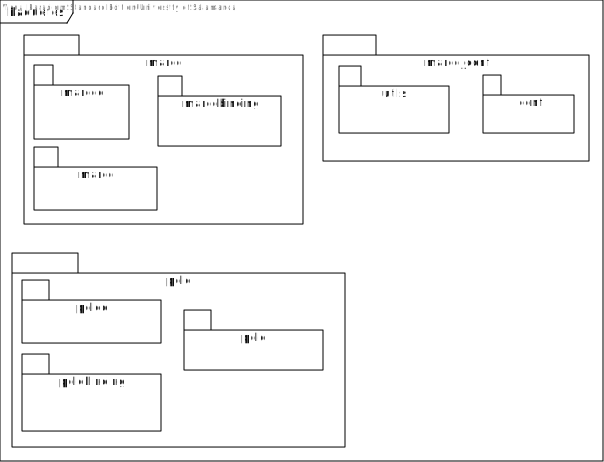
\includegraphics[width=0.6\textwidth]{Paquetes}
\end{figure}

\subsubsection{Paquete Marco}

\begin{figure}[H]
\centering
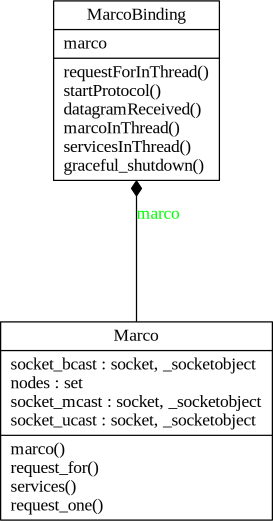
\includegraphics[width=0.2\textwidth]{class_marco_marcobinding}
\end{figure}

\begin{figure}[H]
\centering

\includegraphics[width=0.2\textwidth]{class_marcoexception}
\end{figure}

\subsubsection{Paquete Polo}

\begin{figure}[H]
\centering
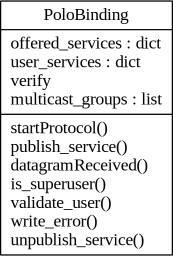
\includegraphics[width=0.2\textwidth]{class_polobinding}
\end{figure}

\begin{figure}[H]
\centering
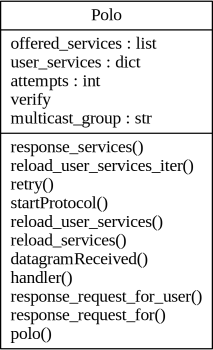
\includegraphics[width=0.2\textwidth]{class_polo}
\end{figure}


\subsubsection{Paquete utils}

\begin{figure}[H]
\centering
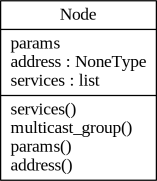
\includegraphics[width=0.2\textwidth]{class_node}
\end{figure}

\subsubsection{Paquete tests}

\begin{figure}[H]
\centering
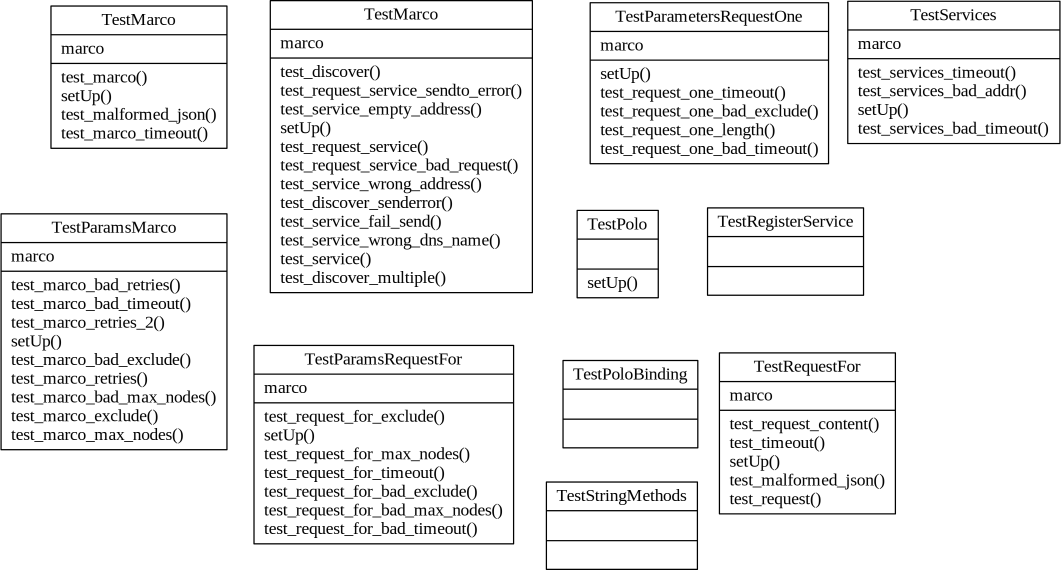
\includegraphics[width=0.2\textwidth]{classes_test}
\end{figure}

\subsection{Vista de interacción}

\subsubsection{Diagramas de comunicación}

\paragraph{Comunicación en Marco}

\begin{figure}[H]
\centering
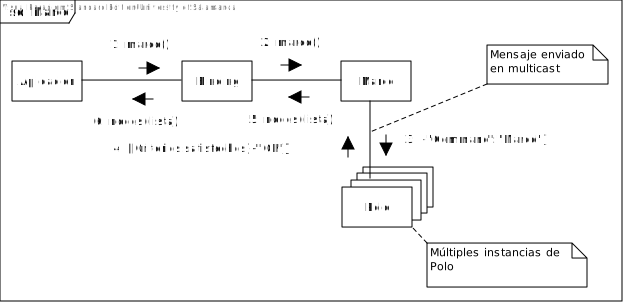
\includegraphics[width=0.6\textwidth]{Marco}
\end{figure}

\paragraph{Comunicación en Polo}

\begin{figure}[H]
\centering
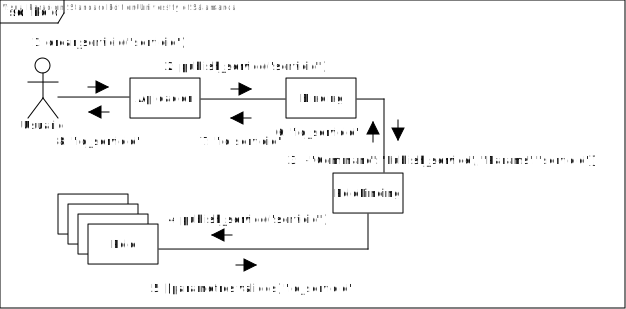
\includegraphics[width=0.6\textwidth]{Polo}
\end{figure}

\subsection{Vista de actividad}

\begin{figure}[H]
\centering
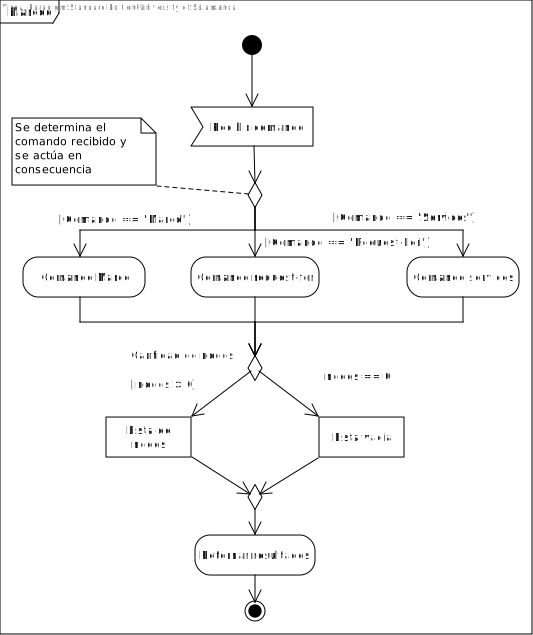
\includegraphics[width=0.7\textwidth]{Marcod}
\end{figure}

\begin{figure}[H]
\centering
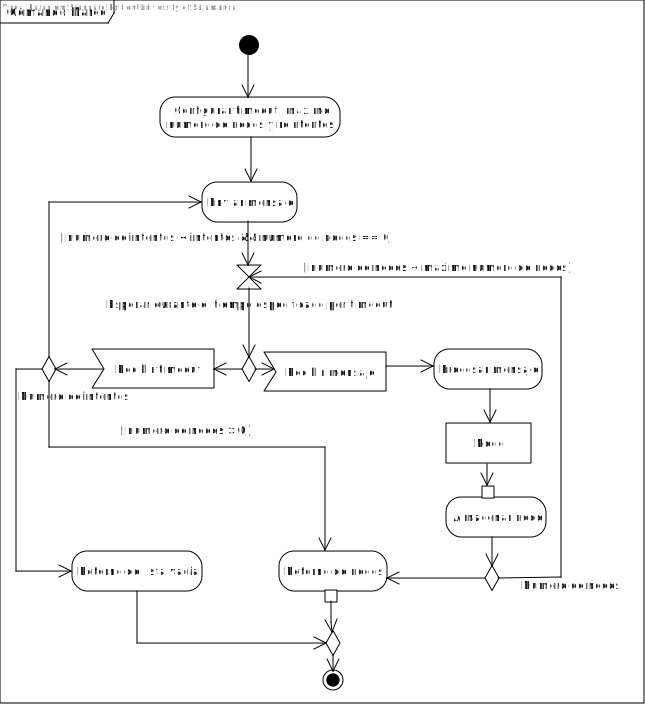
\includegraphics[width=0.7\textwidth]{Comando_Marco}
\end{figure}

\end{document}